\section{Ensemble Methods}
The main idea of ensemble is to combine algorithms to achieve a better accuracy than with a single modell. Ensemble methods can be split into heterogene and homogeneous ensembles. In homogenous ensembles while in heterogen ensembles different algorithms can be combined. 
We implemented homogenous method called adaboost with decision tree stumps(depth=1).    
\begin{figure}[hbtp]
	\centering
	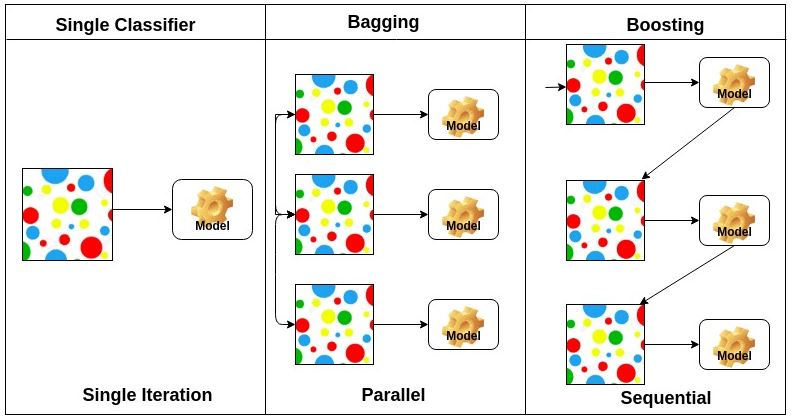
\includegraphics[scale=0.5]{ensemble_1}
	\caption{Bagging/Boosting}
	% \vspace{-20pt}
	\label{fig:Datensatz - unbearbeitet}
\end{figure}

%%%%%%%%%%%%%%%%%%%%%%%%%%%%%%%%%%%%%%%%%%%%%%%%%%%%%%%%%

\subsection{Bagging}


%%%%%%%%%%%%%%%%%%%%%%%%%%%%%%%%%%%%%%%%%%%%%%%%%%%%%%%%%

\subsection{Boosting}


%%%%%%%%%%%%%%%%%%%%%%%%%%%%%%%%%%%%%%%%%%%%%%%%%%%%%%%%%

\subsection{Stacking}


\newpage